% Provenance (never printed): see sources/outline_sources.md (Year 3: the heat
% equation, half-space and plate cooling models, heat flow against age,
% continental geotherms, thermal subsidence). Brief: sources/book5/BRIEFS.md,
% ch. 5. Curves from figdata/bachelor-3/plate_cooling.py (models; Seton et al.
% 2020 age grid and ETOPO1, read only) and continental_geotherm.py.
% Exercise and problem values in the Book 5 scratch calculator calc/ch05.py.
\chapter{岩石圈热模型}\label{ch:b3:lithosphere-thermal-models}

沿洋中脊向外航行，海底逐渐加深：洋脊轴处约
\qty{2.5}{km}，最古老洋底之下则超过 \qty{5}{km}。
板块既未增加物质，也未失去物质，它只是
冷却、收缩并下沉。海底是其下方板块的温度计，
探入沉积物的热流探针从上方读出同样的冷却过程。
本章以两种方式求解板块的冷却问题，即半空间与
厚度有限的板块，并将二者与真实洋底的深度及其热流相比较，
然后转向大陆，
大陆的热量部分来自其自身的地壳。
% ledger: ps77:depth-age

\begin{recall}
热传导的扩散方程 $\partial T/\partial t = \kappa\nabla^2T$，
其中热导率为 $k$，热扩散率 $\kappa =
k/(\rho c)$，属物理学分册的内容；傅里叶级数与误差函数
$\operatorname{erf}x = (2/\sqrt\pi)\int_0^xe^{-u^2}\,\mathrm du$ 见数学大学教材。
热流、放射性生热、
地温线、传导时间尺度 $L^2/\kappa$、热
边界层与热岩石圈在本科一年级分册中定义，
见其中关于地球热收支的一章；地壳均衡见其中关于
均衡与重力异常的一章；深度–年龄关系 $d = d_r + C\sqrt t$ 在其关于
裂谷、洋脊与被动大陆边缘的一章中证明，并在本阶段不加证明地承认
本章推导的温度剖面。盆地的拉伸模型、裂后沉降与
热时间常数见本科二年级分册，
其中关于沉积盆地的一章。
\end{recall}

\section{传导、平流及其比值}

岩石圈中的热量以两种方式传递：一是沿温度梯度
向下扩散，二是随运动的岩石输运，例如板块离开洋脊、
被侵蚀的山隆起、岩浆上升。哪一种占优，取决于一个
单独的数。

\begin{definition}[热佩克莱数]\label{def:b3:lithosphere-thermal-models:peclet}
设岩石以速度 $u$ 穿过长度 $L$，其
\emph{热佩克莱数}\index{热佩克莱数}为
\[
  \mathrm{Pe} = \frac{uL}{\kappa},
\]
即传导时间 $L^2/\kappa$ 与平流时间 $L/u$ 之比。
平流在 $\mathrm{Pe} \gg 1$ 时占优，传导在
$\mathrm{Pe} \ll 1$ 时占优。
\end{definition}

离开洋脊、速度为 \qty{25}{mm/\text{年}} 的板块，在
\qty{95}{km} 的距离上，$\mathrm{Pe} \approx 94$，取 $\kappa = \qty{0.8e-6}{m^2.s^{-1}}$：
热量被板块横向输运的速度远快于其横向扩散。
因此，板块的每个竖直柱体都如同孤立地冷却，
即借竖直方向的传导向冷的海底散热，其年龄 $t$ 表示自其
离开洋脊轴以来的时间。这样，二维问题便化为深度与
时间的一维问题。

\section{冷却半空间}

\begin{definition}[半空间冷却模型]\label{def:b3:lithosphere-thermal-models:half-space}
大洋岩石圈的\emph{半空间冷却模型}\index{半空间冷却模型}将每个柱体
取为热扩散率均匀的半空间 $z \ge 0$，
离开洋脊轴时处于地幔的均匀温度 $T_m$，
其表面此后保持在海底温度 $T_0$，
无生热，也无底边界。
\end{definition}

\begin{theorem}[误差函数地温线]\label{thm:b3:lithosphere-thermal-models:erf}
在\omterm{def:b3:lithosphere-thermal-models:half-space}{半空间冷却模型}中，海底之下深度 $z$ 处的温度
（海底年龄为 $t$）为
\[
  T(z, t) = T_0 + (T_m - T_0)\operatorname{erf}\frac{z}{2\sqrt{\kappa t}} .
\]
此即\emph{误差函数地温线}\index{误差函数地温线}。
\end{theorem}

\begin{proof}
令 $\theta = (T - T_0)/(T_m - T_0)$，它满足 $\partial\theta/\partial t =
\kappa\,\partial^2\theta/\partial z^2$，初始条件 $\theta(z, 0) = 1$（$z > 0$），且
$\theta(0, t) = 0$（$t > 0$）。该问题本身没有长度尺度：
若 $\theta(z, t)$ 为解，则
$\theta(\lambda z, \lambda^2t)$ 对每个 $\lambda > 0$ 亦为解，初值与边值相同。因解唯一，
$\theta$ 依赖于 $z$ 与 $t$，且只通过 $\eta = z/(2\sqrt{\kappa
t})$。记 $\theta = f(\eta)$，并有 $\partial\eta/\partial t = -\eta/(2t)$ 及
$\partial\eta/\partial z = 1/(2\sqrt{\kappa t})$，代入得
\[
  -\frac{\eta}{2t}f'(\eta) = \kappa\,\frac{f''(\eta)}{4\kappa t},
  \qquad\text{故}\qquad f'' + 2\eta f' = 0 .
\]
由此 $f' = Ae^{-\eta^2}$，且 $f = A\int_0^\eta e^{-u^2}\,\mathrm du + B$。
表面条件在 $\eta = 0$ 处给出 $B = 0$；初始条件
在每一深度上，当 $t \to 0$，即 $\eta \to \infty$ 时成立，给出
$A\sqrt\pi/2 = 1$。故 $f = \operatorname{erf}\eta$。
\end{proof}

给定深度处的温度只依赖于 $z/\sqrt t$：等温线
随年龄的平方根下沉，\qty{40}{Ma} 时的冷却层
厚度为 \qty{10}{Ma} 时的两倍。地表热流由求导得出。

\begin{proposition}[热流–年龄关系]\label{prop:b3:lithosphere-thermal-models:heat-flow}
在\omterm{def:b3:lithosphere-thermal-models:half-space}{半空间冷却模型}中，年龄为 $t$ 的海底
之热流为
\[
  q(t) = k\,\frac{\partial T}{\partial z}\Big|_{z=0}
  = \frac{k(T_m - T_0)}{\sqrt{\pi\kappa t}} = \frac{C_q}{\sqrt t} .
\]
\end{proposition}

\begin{proof}
$\partial\operatorname{erf}(z/2\sqrt{\kappa t})/\partial z = (2/\sqrt\pi)
e^{-z^2/4\kappa t}/(2\sqrt{\kappa t})$，在 $z = 0$ 处为 $1/\sqrt{\pi\kappa
t}$。
\end{proof}

下文板块模型的取值（$k = \qty{3.1}{W.m^{-1}.K^{-1}}$，
$T_m - T_0 = \qty{1450}{K}$，$\kappa = \qty{0.8e-6}{m^2.s^{-1}}$），$C_q =
\qty{505}{mW.m^{-2}.Ma^{1/2}}$，接近不同研究对全球测量数据拟合所得的 430 至
\qty{510}{mW.m^{-2}.Ma^{1/2}} 之间的值
；近期一份汇编更倾向于 \num{490}。年轻洋壳上的实测热流
然而严重低估了从洋壳散失的热量：
破裂地壳中循环的海水，把部分热量
经热泉带走，探针无法测得。在老洋壳上，测量值
符合 $1/\sqrt t$，而地球热损失的估计在
年龄小于 \qty{66.5}{Ma} 的洋壳上以 $C_q/\sqrt t$ 代替测量值。
% ledger: honda04:gdh1, b2dd10:half-space, dd10b5:hydrothermal

本科一年级分册通过地壳均衡，对同一剖面沿深度积分，
得到深度–年龄关系 $d = d_r + C\sqrt t$，其中 $C = 2\rho_m\alpha(T_m -
T_0)\sqrt\kappa/\bigl(\sqrt\pi(\rho_m - \rho_w)\bigr)$（见下图）。取
$\rho_m = \qty{3300}{kg.m^{-3}}$，$\rho_w = \qty{1030}{kg.m^{-3}}$ 和 $\alpha =
\qty{3.1e-5}{K^{-1}}$ 时，$C = \qty{370}{m.Ma^{-1/2}}$，
与北太平洋和北大西洋海底拟合所得的 \qty{350}{m.Ma^{-1/2}} 相比，
所用海底的年龄均小于 \qty{70}{Ma}。
% ledger: ps77:depth-age

\begin{omfigure}
\begin{tikzpicture}[font=\small, x=1cm, y=1cm]
% schematic: two columns of equal mass above the compensation depth
\fill[blue!12] (0,0) rectangle (1.6,-1.2);
\fill[orange!35] (0,-1.2) rectangle (1.6,-5.6);
\fill[blue!12] (4.4,0) rectangle (6.6,-2.2);
\shade[top color=blue!35!gray!40, bottom color=orange!35] (4.4,-2.2) rectangle (6.6,-4.4);
\fill[orange!35] (4.4,-4.4) rectangle (6.6,-5.6);
\draw (0,0) rectangle (1.6,-5.6) (4.4,0) rectangle (6.6,-5.6);
\draw[densely dashed] (-0.6,-5.6) -- (7.2,-5.6) node[right, font=\scriptsize] {补偿深度};
\draw[thick] (0,-1.2) -- (1.6,-1.2) (4.4,-2.2) -- (6.6,-2.2);
\node[font=\scriptsize] at (0.8,-0.6) {水};
\node[font=\scriptsize, align=center] at (0.8,-3.4) {地幔 \\于 $T_m$};
\node[font=\scriptsize] at (5.5,-1.1) {水};
\node[font=\scriptsize, align=center] at (5.5,-3.3) {冷却板块 \\$\rho_m(1 + \alpha\,\Delta T)$};
\node[font=\scriptsize, align=center] at (5.5,-5.0) {地幔};
\draw[<->] (-0.3,0) -- (-0.3,-1.2) node[midway, left, font=\scriptsize] {$d_r$};
\draw[<->] (6.9,0) -- (6.9,-2.2) node[midway, right, font=\scriptsize] {$d(t)$};
\node[above, font=\scriptsize] at (0.8,0.05) {洋脊轴};
\node[above, font=\scriptsize] at (5.5,0.05) {年龄 $t$ 的海底};
\draw[gray] (-0.6,0) -- (7.2,0);
\end{tikzpicture}

\par\smallskip{\small 冷却板块的地壳均衡：洋脊处的柱体
与年龄为 $t$ 的柱体在补偿深度以上的质量相同。
冷却、密度增大的板块下沉，水充满其上方的
空间。}\label{fig:b3:lithosphere-thermal-models:columns}
\end{omfigure}

\section{板块模型}

老洋底不再加深：在北太平洋和北大西洋，
深度在 60 至 \qty{80}{Ma} 间偏离 $\sqrt t$ 规律，热流
趋于平稳。半空间会无限冷却下去；必定有某种机制使
板块底部保持温暖。
% ledger: parsons:plate-model

\begin{definition}[板块冷却模型]\label{def:b3:lithosphere-thermal-models:plate}
称大洋岩石圈的\emph{板块冷却模型}\index{板块冷却模型}，即把每一柱体
视为扩散率均匀的一层 $0 \le z \le L$，
在离开洋脊时温度均匀为 $T_m$，其
表面保持在 $T_0$，底部自此起保持在 $T_m$。
\end{definition}

\begin{theorem}[板块模型温度级数]\label{thm:b3:lithosphere-thermal-models:plate-series}
在\omterm{def:b3:lithosphere-thermal-models:plate}{板块冷却模型}中，取 $T_0 = 0$，
\[
  T(z, t) = T_m\Bigl[\frac zL + \frac2\pi\sum_{n=1}^\infty\frac1n
  \sin\frac{n\pi z}{L}\,e^{-n^2t/\tau}\Bigr],\qquad
  \tau = \frac{L^2}{\pi^2\kappa} .
\]
此式称为\emph{板块模型温度级数}\index{板块模型温度级数}。
\end{theorem}

\begin{proof}
稳态在 $t \to \infty$ 时达到，为线性剖面 $T_mz/L$。
偏差 $u = T - T_mz/L$ 满足扩散方程，且 $u = 0$ 于
$z = 0$ 与 $z = L$ 处成立，初值为 $u(z, 0) = T_m(1 - z/L)$。分离
变量，设 $u = Z(z)\Theta(t)$，得 $Z''/Z = \Theta'/(\kappa\Theta) = -\mu^2$；
由边界条件得 $Z = \sin(n\pi z/L)$，$\mu = n\pi/L$，以及
$\Theta = e^{-n^2\pi^2\kappa t/L^2} = e^{-n^2t/\tau}$。由初值确定
$b_n$ 为 $T_m(1 - z/L)$ 在 $[0, L]$ 上正弦级数的系数：
\[
  b_n = \frac2L\int_0^LT_m\Bigl(1 - \frac zL\Bigr)\sin\frac{n\pi z}{L}\,\mathrm dz
  = \frac{2T_m}{n\pi},
\]
由分部积分可得。对各模式求和即得级数。
\end{proof}

各模式以其自身的时间 $\tau/n^2$ 衰减：高次谐波，即
初始阶跃的精细结构最先消失，经过量级为 $\tau$ 的时间后
只剩第一项。用同样的分离变量法可得热流，
并借助上图的均衡关系得到深度。

\begin{proposition}[板块模型的深度与热流]\label{prop:b3:lithosphere-thermal-models:plate-depth}
在\omterm{def:b3:lithosphere-thermal-models:plate}{板块冷却模型}中，沿用深度–年龄
关系中的密度与热膨胀系数，
\[
  q(t) = \frac{kT_m}{L}\Bigl[1 + 2\sum_{n=1}^\infty e^{-n^2t/\tau}\Bigr],\qquad
  d(t) = d_r + \frac{\rho_m\alpha T_mL}{2(\rho_m - \rho_w)}
  \Bigl[1 - \frac{8}{\pi^2}\sum_{n\ \text{奇数}}\frac{e^{-n^2t/\tau}}{n^2}\Bigr].
\]
当 $t \to \infty$ 时，深度趋于 $d_r + \rho_m\alpha T_mL/\bigl(2(\rho_m -
\rho_w)\bigr)$，热流趋于 $kT_m/L$，二者均指数地趋近，
时间常数为 $\tau$。
\end{proposition}

\begin{proof}
对级数在 $z = 0$ 处求导，$\partial T/\partial z = (T_m/L)[1 +
2\sum e^{-n^2t/\tau}]$。对深度，由均衡条件 $(\rho_m -
\rho_w)(d - d_r) = \rho_m\alpha\int_0^L(T_m - T)\,\mathrm dz$。线性部分
贡献 $T_mL/2$；每个模态贡献 $-(2T_m/n\pi)e^{-n^2t/\tau}
\int_0^L\sin(n\pi z/L)\,\mathrm dz = -(2T_m/n\pi)(L/n\pi)(1 - \cos n\pi)
e^{-n^2t/\tau}$，偶数 $n$ 时为零，奇数时为 $-(4T_mL/n^2\pi^2)
e^{-n^2t/\tau}$（$n$ 为奇数）。提出 $T_mL/2$ 即得括号内的式子。当 $t = 0$
时该式为零，因为 $\sum_{n\ \text{奇数}}1/n^2 = \pi^2/8$。
\end{proof}

最佳拟合全球深度与热流的板块模型，板块厚度为
\qty{95}{km}，底部温度为 \qty{1450}{\celsius}，$\alpha =
\qty{3.1e-5}{K^{-1}}$，$k = \qty{3.1}{W.m^{-1}.K^{-1}}$，
比早先的 \qty{125}{km}、\qty{1350}{\celsius} 更薄、更热。取 $\kappa =
\qty{0.8e-6}{m^2.s^{-1}}$，$\tau = \qty{36.2}{Ma}$；深度趋于
$2500 + 3104 = \qty{5604}{m}$，热流趋于 \qty{47}{mW.m^{-2}}。年轻的
海底无法区分这两种模型：二者在 \qty{2}{Ma} 时相差不到一米，
在 \qty{44}{Ma} 时相差达 \qty{100}{m}。地震学也给出相近的结论：
太平洋\omterm{def:b3:seismology-imaging:surface-waves}{瑞利波}以渐近厚度为
85 至 \qty{95}{km} 的冷却板块拟合最好。
% ledger: honda04:gdh1, ps77:depth-age, fischer:lithosphere

\begin{omfigure}
\begin{tikzpicture}
\begin{groupplot}[group style={group size=1 by 2, vertical sep=2.3cm},
  omrecord, width=0.86\linewidth, height=0.42\linewidth, xmin=0, xmax=160,
  xlabel={海底年龄 (Ma)}]
\nextgroupplot[omdepth, ylabel={深度 (km)}, ymin=0, ymax=130,
  title={(a) 等温线，每隔 \qty{200}{\celsius}}, title style={font=\small},
  legend style={font=\scriptsize, at={(0.01,0.03)}, anchor=south west}]
% computed in figdata/bachelor-3/plate_cooling.py; ledger: honda04:gdh1
\addplot[omDef, thick] table[x=t, y=hs200] {figdata/out/bachelor-3-plate_cooling-isotherms.dat};
\addlegendentry{半空间}
\addplot[red!70!black, thick, densely dashed] table[x=t, y=pl200] {figdata/out/bachelor-3-plate_cooling-isotherms.dat};
\addlegendentry{板块，$L = \qty{95}{km}$}
\foreach \lev in {400,600,800,1000,1200,1400} {
  \addplot[omDef, thick, forget plot] table[x=t, y=hs\lev] {figdata/out/bachelor-3-plate_cooling-isotherms.dat};
  \addplot[red!70!black, thick, densely dashed, forget plot] table[x=t, y=pl\lev] {figdata/out/bachelor-3-plate_cooling-isotherms.dat};
}
\draw[gray] (axis cs:0,95) -- (axis cs:160,95);
\node[font=\scriptsize, anchor=north] at (axis cs:68,96) {板块底部};
\node[font=\scriptsize, fill=white, inner sep=1pt] at (axis cs:150,14) {200};
\node[font=\scriptsize, fill=white, inner sep=1pt] at (axis cs:28,38.2) {1000};
\node[font=\scriptsize, fill=white, inner sep=1pt] at (axis cs:22,70.4) {1400};
\nextgroupplot[ylabel={热流 (\unit{mW.m^{-2}})}, ymin=0, ymax=300,
  title={(b) 热流}, title style={font=\small},
  legend style={font=\scriptsize, at={(0.98,0.97)}, anchor=north east}]
\addplot[omDef, thick] table[x=t, y=hs] {figdata/out/bachelor-3-plate_cooling-heat.dat};
\addlegendentry{半空间}
\addplot[red!70!black, thick, densely dashed] table[x=t, y=pl] {figdata/out/bachelor-3-plate_cooling-heat.dat};
\addlegendentry{板块}
\end{groupplot}
\end{tikzpicture}

\par\smallskip{\small 两种冷却模型，参数取自正文。
(a) 各等温线的深度，从 \qty{200}{\celsius}（顶部）到
\qty{1400}{\celsius}（底部）：半空间中的深度随
$\sqrt t$ 增加而继续下沉，板块中的深度则在剖面变为线性时趋于稳定。(b) 地表
热流：板块模型趋于 \qty{47}{mW.m^{-2}}，半空间模型
按 $1/\sqrt t$ 下降。}\label{fig:b3:lithosphere-thermal-models:isotherms}
\end{omfigure}

实际的海底可以放在同一张图上（见下图）。每个
纬度与经度各一度、年龄已知的网格单元，都按其年龄和深度标在图上；
每个五百万年区间内深度的中位数随年龄增加，
在前 \qty{40}{Ma} 内与模型所示一致，但观测的海底比两个模型都浅，
且年龄越大，偏离越明显。未作任何校正：老海底覆着更厚的
沉积层，较老的北大西洋中超过一千米，
其重量使海底下沉，并抬高其顶面；老海底还有足够的时间
积累海山、火山高原和热点隆起。已发表的
拟合首先去除沉积物负荷和明显的隆起。本科一年级分册中的深度--
年龄关系，以及上面的板块模型，都来自这样校正后的
深度。
% ledger: data:b5-depth-age, ps77:depth-age

\begin{omfigure}
\begin{tikzpicture}
\begin{axis}[omrecord, omdepth, width=0.86\linewidth, height=0.5\linewidth,
  xmin=0, xmax=180, ymin=2, ymax=6.5, xlabel={海底年龄 (Ma)},
  ylabel={深度 (km)},
  legend style={font=\scriptsize, at={(0.5,-0.24)}, anchor=north, cells={anchor=west}},
  legend columns=2]
% computed in figdata/bachelor-3/plate_cooling.py; ledger: data:b5-depth-age, honda04:gdh1
\addplot[only marks, mark=*, mark size=1.3pt, black,
  error bars/.cd, y dir=both, y explicit]
  table[x=t, y expr=\thisrow{med}/1000, y error plus expr=(\thisrow{q3}-\thisrow{med})/1000,
  y error minus expr=(\thisrow{med}-\thisrow{q1})/1000] {figdata/out/bachelor-3-plate_cooling-bins.dat};
\addlegendentry{观测值，中位数与四分位数}
\addplot[omDef, thick] table[x=t, y expr=\thisrow{hs}/1000] {figdata/out/bachelor-3-plate_cooling-depth.dat};
\addlegendentry{半空间}
\addplot[red!70!black, thick, densely dashed] table[x=t, y expr=\thisrow{pl}/1000] {figdata/out/bachelor-3-plate_cooling-depth.dat};
\addlegendentry{板块，$L = \qty{95}{km}$}
\end{axis}
\end{tikzpicture}

\par\smallskip{\small 海底深度随年龄的变化：中位数与
四分位数，即各五百万年区间内一度×一度网格单元的深度
区间（仅计入深于 \qty{1000}{m} 的海底，年龄取自全球年龄网格，
深度取自全球地形模型，未校正沉积物、海山或隆起），
并与正文中的两种冷却模型对比。}\label{fig:b3:lithosphere-thermal-models:depth-age}
\end{omfigure}

\begin{definition}[热沉降]\label{def:b3:lithosphere-thermal-models:thermal-subsidence}
\emph{热沉降}\index{热沉降}是指岩石圈表面的
在冷却、收缩并趋向热平衡时发生的下沉，其上方
空间由水或沉积物充填；地壳均衡将
一柱岩石失去的热量转化为该柱的下沉。
\end{definition}

海底是最纯粹的情形。另一例是拉伸的大陆盆地：
岩石圈按因子 $\beta$ 减薄，使热的软流圈上升，而
本科二年级分册中的裂后沉降本质上是同一板块冷却过程，只是起始
剖面不同，具有相同的模态与相同的衰减时间 $\tau/n^2$。
因此，待高阶模态衰减之后，仅保留第一模态是较好的近似，
而在此之前则较差：对于上文板块模型的海底，
仅取第一项，在 \qty{20}{Ma} 后给出的深度误差在两米以内，
但在 \qty{5}{Ma} 时深度偏大 \qty{84}{m}。

\section{大陆地温线}

大陆地壳会产生热量：花岗岩中含有铀、钍和钾，
其浓度使上地壳产热占到地表热流的很大一部分。
产热量随深度如何分布，
决定了深部的温度。

\begin{definition}[生热深度尺度；折合热流]\label{def:b3:lithosphere-thermal-models:reduced}
当地壳的放射性生热随深度按
$A(z) = A_0e^{-z/h_r}$ 递减时，$h_r$ 称为
\emph{生热深度尺度}\index{生热深度尺度}。某一省的
\emph{折合热流}\index{折合热流}$q_m$ 是指若地壳不产热，
其地表处仍会保留的热流，即
放射性层以下传来的热流。
\end{definition}

\begin{proposition}[指数型生热]\label{prop:b3:lithosphere-thermal-models:exponential}
在稳态传导中，导热率 $k$ 均匀，地表温度为 $0$，
生热率为 $A_0e^{-z/h_r}$，深部热流为 $q_m$，则
地表热流为
\[
  q_0 = q_m + A_0h_r,
\]
地温线为
\[
  T(z) = \frac{q_mz}{k} + \frac{A_0h_r^2}{k}\bigl(1 - e^{-z/h_r}\bigr).
\]
若某一省的深成岩体具有相同的 $h_r$ 与相同的 $q_m$，则其
地表热流与地表生热率位于同一直线
上，即 $q_0 = q_m + h_rA_0$。
\end{proposition}

\begin{proof}
稳态时，向上的热流 $q(z) = k\,\mathrm dT/\mathrm dz$
因产热而逐渐减小：$\mathrm dq/\mathrm dz = -A(z)$。当深部 $q \to q_m$ 时，
有 $q(z) = q_m + A_0h_re^{-z/h_r}$，故 $q_0 = q_m + A_0h_r$。积分
$\mathrm dT/\mathrm dz = q(z)/k$ 并由 $T(0) = 0$ 积分即得地温线。末
一句即为前一结论对每个深成岩体的应用。
\end{proof}

这一直线已被观测证实：在若干省份中，深成岩体的热流与地表生热率
落在直线上，\omterm{def:b3:lithosphere-thermal-models:reduced}{生热深度尺度}为 7.5 至
\qty{10}{km}，\omterm{def:b3:lithosphere-thermal-models:reduced}{折合热流}为 \qty{0.8}{HFU}（约
\qty{33.5}{mW.m^{-2}}），位于落基山脉以东。指数形式并非
唯一能给出直线的形式，但它在侵蚀作用下仍保持直线：自顶部移去厚度为 $e$ 的一层，会使
$A_0$ 与 $q_0$ 的放射性部分乘以同一因子 $e^{-e/h_r}$。
% ledger: b2roy:provinces

下图给出地表热流分别为 40、60 和
\qty{80}{mW.m^{-2}} 的地温线，其中前者典型于克拉通，后者典型于弧后区，
并取 $k = \qty{2.5}{W.m^{-1}.K^{-1}}$、$h_r = \qty{10}{km}$，地壳份额
为 $A_0h_r = 0.4\,q_0$。取 \qty{1300}{\celsius} 等温线作为
热岩石圈底界，其深度分别为 129、84 和 \qty{61}{km}。
地震学表明，克拉通地幔的高速区延伸至约 \qty{250}{km}，弧后岩石圈
厚 50 至 \qty{60}{km}。克拉通冷而厚的根部所需的
\omterm{def:b3:lithosphere-thermal-models:reduced}{折合热流}比该简单模型所给出的更小，且其
导热率随温度变化，但对比的数量级是对的。
% ledger: hyndman:backarc, fischer:lithosphere, delaney86:properties

\begin{omfigure}
\begin{tikzpicture}
\begin{axis}[omrecord, omdepth, width=0.62\linewidth, height=0.6\linewidth,
  xmin=0, xmax=1600, ymin=0, ymax=200, xlabel={温度 (\unit{\celsius})},
  ylabel={深度 (km)},
  legend style={font=\scriptsize, at={(0.02,0.03)}, anchor=south west, cells={anchor=west}}]
% computed in figdata/bachelor-3/continental_geotherm.py
\addplot[black, thick] table[x=T40, y=z] {figdata/out/bachelor-3-continental_geotherm-geotherms.dat};
\addlegendentry{$q_0 = \qty{40}{mW.m^{-2}}$}
\addplot[omDef, thick, densely dashed] table[x=T60, y=z] {figdata/out/bachelor-3-continental_geotherm-geotherms.dat};
\addlegendentry{$q_0 = \qty{60}{mW.m^{-2}}$}
\addplot[red!70!black, thick, dashdotted] table[x=T80, y=z] {figdata/out/bachelor-3-continental_geotherm-geotherms.dat};
\addlegendentry{$q_0 = \qty{80}{mW.m^{-2}}$}
\draw[gray, densely dotted] (axis cs:1300,0) -- (axis cs:1300,200);
\node[font=\scriptsize, rotate=90, anchor=south] at (axis cs:1300,160) {\qty{1300}{\celsius}};
\end{axis}
\end{tikzpicture}

\par\smallskip{\small 稳态大陆地温线，生热率随深度指数递减
（$h_r = \qty{10}{km}$，$A_0h_r = 0.4\,q_0$，$k =
\qty{2.5}{W.m^{-1}.K^{-1}}$），对应三种地表热流。近地表的曲率
反映的是地壳自身的产热；在若干个深度尺度以下，每条地温线
均为梯度为 $q_m/k$ 的直线。}\label{fig:b3:lithosphere-thermal-models:geotherms}
\end{omfigure}

\begin{inthefield}[海上测量热流]
\begin{minipage}[t]{0.55\linewidth}\vspace{0pt}
海洋热流探针是一根长钢杆，顶端压有重块，
杆侧沿一细管布置有温度传感器。从科考船的
船尾用绞车缆绳将其放至海底，任其
自由落入软沉积物中，传感器一并入泥。探针静止数分钟，
待插入过程产生的摩擦热散去，传感器稳定在
周围泥浆的温度。相隔数米的各读数即可给出
温度梯度。随后沿管发出一短促热脉冲，
其衰减速率即给出周围沉积物的导热率，
两者之积即为热流。钢杆拔出后，
在测线上再前移数百米重新放下，不必回收到
甲板上。
\end{minipage}\hfill
\begin{minipage}[t]{0.42\linewidth}\vspace{0pt}
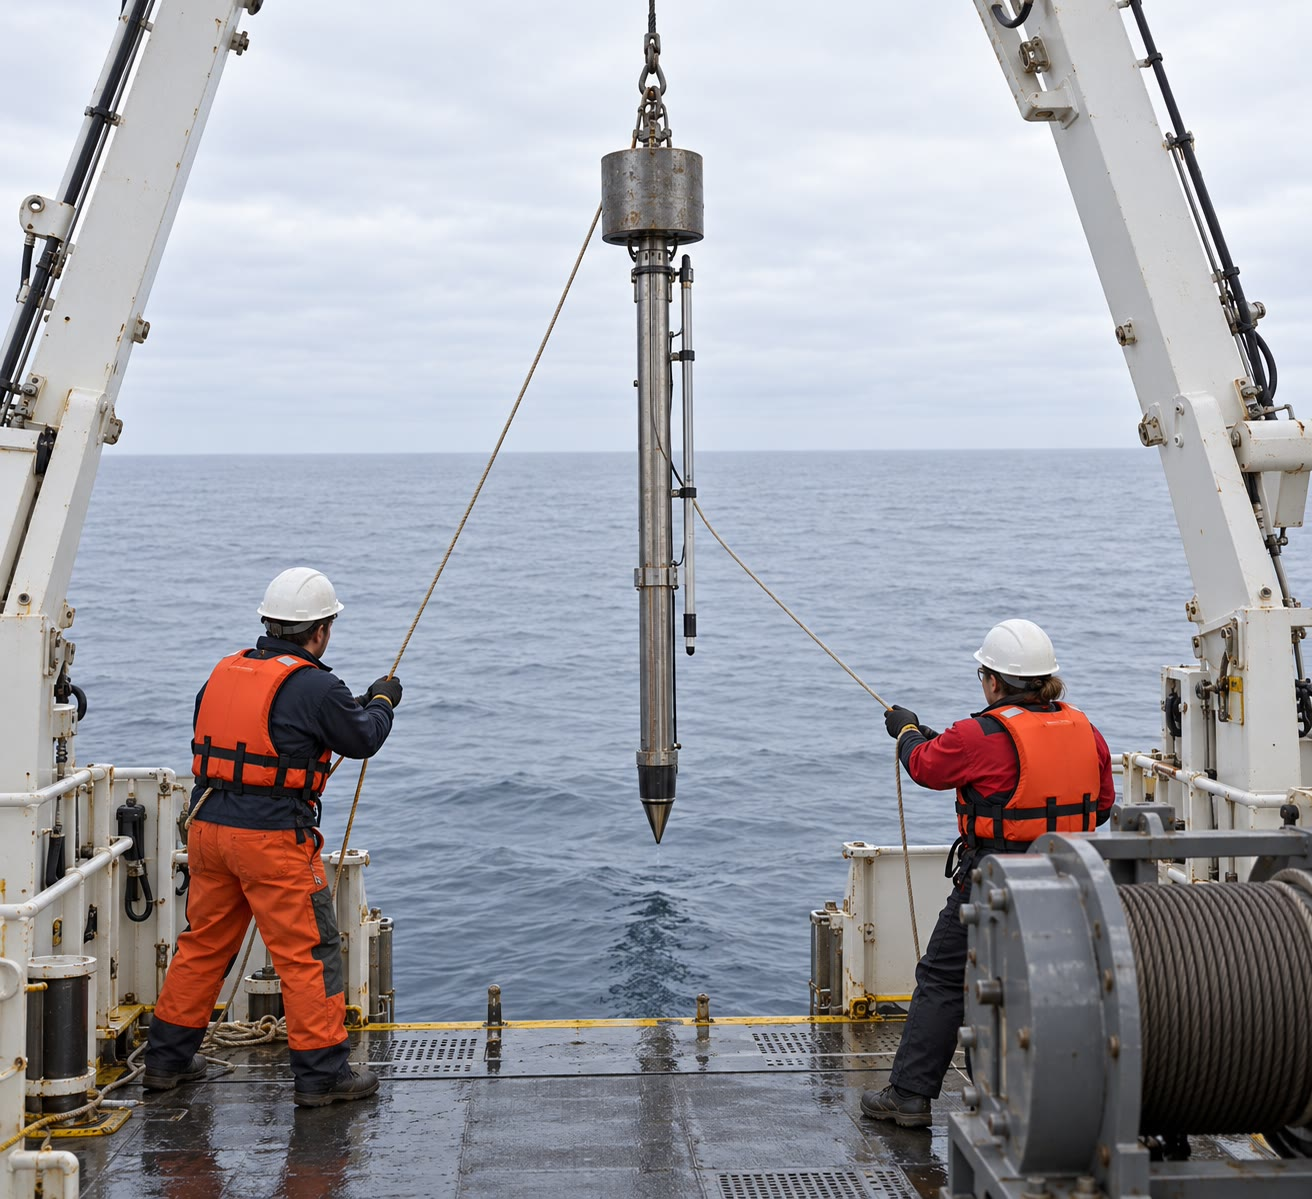
\includegraphics[width=\linewidth]{images/book5/ai/b3-heatflow-probe.jpg}

{\scriptsize 研究船船尾即将放下的热流探针
（AI 生成插图）。}
\end{minipage}
\end{inthefield}

\section{练习}

\begin{exercise}[$\star$]\label{exo:b3:lithosphere-thermal-models:1}
取 $\kappa = \qty{e-6}{m^2.s^{-1}}$，计算传导时间 $L^2/\kappa$，
分别对 $L = 1$、10 和 \qty{100}{km}，以百万年为单位。
\end{exercise}

\begin{exercise}[$\star$]\label{exo:b3:lithosphere-thermal-models:2}
某山脉以 \qty{1}{mm/\text{年}} 的速率被侵蚀，岩石需从上部
\qty{30}{km} 厚的地壳中上升以补偿其损失。取 $\kappa = \qty{e-6}{m^2.s^{-1}}$，
计算佩克莱数。该山脉的地温线能否仅由
传导算出？
\end{exercise}

\begin{exercise}[$\star$]\label{exo:b3:lithosphere-thermal-models:3}
在半空间模型（$T_0 = 0$，$T_m = \qty{1450}{\celsius}$，$\kappa =
\qty{0.8e-6}{m^2.s^{-1}}$）中，计算海底以下 \qty{10}{km} 处的温度，
海底年龄为 \qty{5}{Ma}（\qty{1}{Ma} $= \qty{3.156e13}{s}$；$\operatorname{erf}
0.445 = 0.471$）。
\end{exercise}

\begin{exercise}[$\star$]\label{exo:b3:lithosphere-thermal-models:4}
取 $C_q = \qty{490}{mW.m^{-2}.Ma^{1/2}}$，计算年龄为
1、25 和 \qty{100}{Ma} 的海底的热流。三者中，探针
最可能低估哪一个？
\end{exercise}

\begin{exercise}[$\star\star$]\label{exo:b3:lithosphere-thermal-models:5}
在半空间模型中，温度达到 $T_m$ 的 \qty{90}{\percent} 时
对应 $\operatorname{erf}\eta = 0.9$，$\eta = 1.163$。取 $\kappa =
\qty{0.8e-6}{m^2.s^{-1}}$，计算年龄为 10、40 和 \qty{100}{Ma} 时的该深度。
\end{exercise}

\begin{exercise}[$\star\star$]\label{exo:b3:lithosphere-thermal-models:6}
利用正文中的数值，半空间模型给出 $C =
\qty{370.5}{m.Ma^{-1/2}}$。保持其他量不变，热膨胀系数取何值
才能得到拟合值 \qty{350}{m.Ma^{-1/2}}？还可以
改变哪一个参数来代替？
\end{exercise}

\begin{exercise}[$\star\star$]\label{exo:b3:lithosphere-thermal-models:7}
计算板块模型的渐近热流 $kT_m/L$，取 $L =
\qty{95}{km}$，$T_m = \qty{1450}{\celsius}$；以及 $L = \qty{125}{km}$，
$T_m = \qty{1350}{\celsius}$，两种情形下均取 $k = \qty{3.1}{W.m^{-1}.K^{-1}}$。
二者中哪一个更接近由 $C_q/\sqrt t$ 算得的老洋底热流，
即在 \qty{150}{Ma} 处取 $C_q = \qty{490}{mW.m^{-2}.Ma^{1/2}}$ 所得的热流？
\end{exercise}

\begin{exercise}[$\star\star$]\label{exo:b3:lithosphere-thermal-models:8}
某省份有 $q_0 = \qty{60}{mW.m^{-2}}$，$h_r = \qty{10}{km}$，且 $A_0h_r =
0.4\,q_0$。计算 $A_0$、$q_m$ 以及莫霍面处的温度，
莫霍面深 \qty{35}{km}，取 $k = \qty{2.5}{W.m^{-1}.K^{-1}}$。
\end{exercise}

\begin{exercise}[$\star\star$]\label{exo:b3:lithosphere-thermal-models:9}
同一省份的两个花岗岩深成岩体给出 $q_0 = \qty{66}{mW.m^{-2}}$，$A_0
= \qty{3.0}{\micro W.m^{-3}}$；以及 $q_0 = \qty{48}{mW.m^{-2}}$，$A_0 =
\qty{1.2}{\micro W.m^{-3}}$。假设二者都位于
\cref{prop:b3:lithosphere-thermal-models:exponential} 的直线上，计算 $h_r$ 和 $q_m$。
\end{exercise}

\begin{exercise}[$\star\star\star$]\label{exo:b3:lithosphere-thermal-models:10}
(a) 证明在半空间模型中，海底在年龄 0 至 $t$ 之间
单位面积损失的热量为 $Q(t) = 2k(T_m - T_0)\sqrt{t/(\pi\kappa)}$。
(b) 证明沉降量为 $d - d_r = \alpha Q/\bigl(c(\rho_m -
\rho_w)\bigr)$，其中 $c = k/(\rho_m\kappa)$ 为比热容。(c) 对其做数值检验，
在 \qty{40}{Ma} 处，取正文中的数值。
\end{exercise}

\begin{exercise}[$\star\star\star$]\label{exo:b3:lithosphere-thermal-models:11}
在正文的板块模型中（$\tau = \qty{36.2}{Ma}$，$\rho_m\alpha T_mL/
\bigl(2(\rho_m - \rho_w)\bigr) = \qty{3104}{m}$），仅取第一项傅里叶项所算得的深度，
超出完整级数的部分主要来自 $n = 3$ 项。
计算该项在 1、10 和 \qty{20}{Ma} 时的大小，以及
使仅用第一项与级数之差在 \qty{10}{m} 以内的年龄。
\end{exercise}

\begin{exercise}[$\star\star\star$]\label{exo:b3:lithosphere-thermal-models:12}
(a) 证明在 \cref{prop:b3:lithosphere-thermal-models:exponential} 的地温线中，
$T(z) \approx q_mz/k + A_0h_r^2/k$，当 $z \gg h_r$ 时成立。(b) 由此推出
当 $q_0 = \qty{40}{mW.m^{-2}}$ 时 \qty{1300}{\celsius} 等温线的深度，取
练习 8 中的数值。(c) 若要使该深度达到
\qty{250}{km}（即克拉通快速根的深度），$q_m$ 需降低多少？
\end{exercise}

\section{问题：离开洋脊的四千万年}

\begin{problem}[{周末问题 --- 半空间与板块，虚构海洋的深度
及其板块的厚度}]
\label{pb:b3:lithosphere-thermal-models:1}
% values: calc/ch05.py; plate_cooling.py; honda04:gdh1, ps77:depth-age, data:b5-depth-age
取 $T_0 = 0$，$T_m = \qty{1450}{\celsius}$，$\kappa =
\qty{0.8e-6}{m^2.s^{-1}}$，$k = \qty{3.1}{W.m^{-1}.K^{-1}}$，$\alpha =
\qty{3.1e-5}{K^{-1}}$，$\rho_m = \qty{3300}{kg.m^{-3}}$，$\rho_w =
\qty{1030}{kg.m^{-3}}$，洋脊深 \qty{2500}{m}，并取 \qty{1}{Ma} $=
\qty{3.156e13}{s}$。

\medskip\noindent\textbf{第一部分 --- 半空间。}
\begin{enumerate}
  \item 计算 10 和 \qty{40}{Ma} 时的 $\sqrt{\kappa t}$。
  \item 计算两个年龄下海底以下 \qty{20}{km} 处的温度
        （$\operatorname{erf}0.6294 = 0.6266$，$\operatorname{erf}0.3147 =
        0.3437$）。
  \item \qty{1000}{\celsius} 等温线位于 $\operatorname{erf}\eta =
        0.6897$，$\eta = 0.7174$。计算两个年龄下的深度，以及
        它达到 \qty{60}{km} 时的年龄。
  \item 计算两个年龄下的热流，以及 $C_q$。
  \item 一条洋脊两侧各以 \qty{25}{mm/\text{年}} 的速率扩张。计算
        \qty{95}{km} 范围内板块的佩克莱数。为何每一列可以
        单独冷却？
  \item 计算穿过 \qty{95}{km} 的传导时间。对于
        年龄为 \qty{150}{Ma} 的海底，半空间模型说明了什么？
\end{enumerate}

\medskip\noindent\textbf{第二部分 --- 沉降。}
\begin{enumerate}[resume]
  \item 回顾把柱体温度亏损转化为沉降的地壳均衡关系，
        以及为何在半空间中
        可将积分上限取为无穷。
  \item 计算深度–年龄关系中的 $C$，以及 10 和
        \qty{40}{Ma} 处的深度。
  \item 40 至 \qty{45}{Ma} 之间真实洋底的中位深度
        为 \qty{4475}{m}，未作修正。将其与 \qty{42.5}{Ma}
        处的模型相比较，并列出中位数包含而模型
        未予考虑的内容。
  \item $C$ 将变化多少，若 $T_m$ 取 \qty{1350}{\celsius}？
        与拟合得到的 \qty{350}{m.Ma^{-1/2}} 相比较。
  \item 为何年轻洋底上实测的热流低于 $C_q/\sqrt t$？
\end{enumerate}

\medskip\noindent\textbf{第三部分 --- 板块。}取 $L = \qty{95}{km}$。
\begin{enumerate}[resume]
  \item 计算 $\tau$ 及振幅 $\rho_m\alpha T_mL/\bigl(2(\rho_m -
        \rho_w)\bigr)$。
  \item 计算 \qty{40}{Ma} 处的深度，取 $n = 1$、3 和 5 项。
  \item 仅取第一项时，它与上述结果相差多少，
        以及为何差异如此之小？
  \item 计算半空间与板块在 40 和
        \qty{50}{Ma} 处的深度之差，并用线性插值估计该差值达到
        \qty{100}{m} 时的年龄。
  \item 计算 \qty{40}{Ma} 处板块的热流，取
        $n = 1$ 至 3 项，并与半空间相比较。
  \item 给出渐近深度和热流。
\end{enumerate}

\medskip\noindent\textbf{第四部分 --- 一个虚构的大洋。}在一个虚构的大洋中，
其洋脊深 \qty{2500}{m}，洋底经沉积校正并远离海山与隆起后，
深度在 \qty{120}{Ma} 时为 \qty{5700}{m}，在
\qty{40}{Ma} 时为 \qty{4800}{m}。板块的 $L$ 未知；其余
各值均同上。
\begin{enumerate}[resume]
  \item 仅保留第一项傅里叶级数，写出
        \qty{120}{Ma} 处的深度作为 $L$ 的函数，其中
        $\tau$ 本身亦依赖于 $L$。
  \item 用迭代法求解 $L$，初值取 $L = \qty{100}{km}$：
        先计算 $\tau$，再求与 \qty{5700}{m} 相符的 $L$，
        然后用该 $\tau$ 重复迭代。
  \item 取所求得的 $L$，计算 \qty{40}{Ma} 处的深度，
        并与半空间结果及实测的 \qty{4800}{m} 相比较。
  \item 计算 $\tau$（对应该 $L$），以及该大洋的渐近深度。
  \item 洋底的深度在何年龄之后，与其渐近深度
        之差已在 \qty{100}{m} 以内？
  \item 给出拟合该虚构大洋古老洋底的板块
        厚度 $L$。
\end{enumerate}
\end{problem}
